\documentclass{article}
\usepackage{polski}
\usepackage[utf8]{inputenc}
\usepackage{float}
\usepackage{graphicx}
\usepackage{caption}
\usepackage{subcaption}
\usepackage{ragged2e}
\usepackage{amsmath}
\usepackage{blindtext}
\usepackage{hyperref}
\usepackage{algorithmicx}
\usepackage{algpseudocode}
\usepackage{listings}
\usepackage{booktabs}
\usepackage{siunitx}
\usepackage{multicol}
\usepackage{fancyvrb}
\begin{document}

\AddToHook{cmd/section/before}{\clearpage}

\section*{Zadanie 1}
W zadaniu pierwszym mamy przy pomocy Julii wyznaczyć
iteracyjnie kilka wartości powiązanych z liczbami zmiennoprzecinkowymi.
\subsection*{Obliczanie Macheps}
$Macheps$ (epsilon maszynowy) to odległość między liczbą $1.0$ i jej następnikiem
w systemie liczb zmiennopozycyjnych.
Sam algorytm, którym szukałem tej wartości polegał na wykonywaniu dzielenia $x / 2$ dopóki
$1.0 + x > 1.0$ zaczynając od $x = 1.0$ i zwracając ostatnią wartość, która nie spełnia
warunku pętli. Poniżej wyniki:
\begin{table}[h]
    \centering
    \begin{tabular}{|c|c|c|c|}
      \hline
      & float16 & float32 & float64 \\
      \hline
      moje obliczenia &0.000977&1.1920929e-7&2.220446049250313e-16\\
      \hline
      Julia &0.000977&1.1920929e-7&2.220446049250313e-16\\
      \hline
      float.h &?&1.192093e-07&2.220446e-16\\
      \hline
    \end{tabular}
    \caption{Porównanie obliczonego $macheps$}
  \end{table}\\
Nie udało mi się znaleźć w nagłówku float.h wartości dla 16-bitowego floata,
na moim systemie $float$ ma $32$ bity, $double$ ma $64$ bity, a $long\ double$ ma $128$ bit.
Poza tym wyniki się zgadzają między wszystkimi trzema źródłami.
\subsection*{Obliczanie Eta}
$Eta$ to odległość między liczbą 0.0, a jej następnikiem.
Algorytm szukania $eta$, którego użyłem jest analogiczny do tego, którym
szukałem $macheps$ z tą różnicą, że zamiast $1.0 + x > 1.0$ jest $0.0 + x > 0.0$. 
Poniżej wyniki:
\begin{table}[h]
    \centering
    \begin{tabular}{|c|c|c|c|}
      \hline
      & float16 & float32 & float64 \\
      \hline
      moje obliczenia &6.0e-8&1.0e-45&5.0e-324\\
      \hline
      Julia &6.0e-8&1.0e-45&5.0e-324\\
      \hline
    \end{tabular}
    \caption{Porównanie obliczonego $eta$}
  \end{table}\\
Wyniki są poprawne z tą uwagą, że widać wyniki iż są zaokrąglone,
co wynika jednak ze sposobu w jaki Julia
je wypisuje, a mianowicie wywołująć funkcję printf z libc.
\subsection*{Obliczanie Maximum}
$Max$ to największa liczba zmiennoprzecinkowa, która nie jest równa $\infty$.
Algorytm szukający tej wartości wymaga znajomości reprezentacji bitowej liczb
w formacie IEE 754. W wypadku wartości $Max$, jest ona wypełniona $1$ na wszystkich
pozycjach poza bitem znaku i najmłodszym bitem wykładnika. Aby znaleźć tę liczbę, 
najprościej będzie nam najpierw wziąć jakąś znormalizowaną liczbę, której mantysa
składa się z samych $1$, a następnie mnożyć ją przez $2$. Największa taka liczba
różna od $\infty$ jest właśnie naszym $Max$. W moim wypadku szukam liczby odpowiadającej
prevfloat(1.0), ponieważ potęgi $2$ mają same $0$ w mantysie, więc liczba poprzednia
musi mieć same $1$.
\begin{table}[h]
    \centering
    \begin{tabular}{|c|c|c|c|}
      \hline
      & float16 & float32 & float64 \\
      \hline
      moje obliczenia &6.55e4&3.4028235e38&1.7976931348623157e308\\
      \hline
      Julia &6.55e4&3.4028235e38&1.7976931348623157e308\\
      \hline
    \end{tabular}
    \caption{Porównanie obliczonego $Max$}
  \end{table}\\
\subsection*{Związek Macheps z precyzją arytmetyki}
Liczba $Macheps$ to odległość między $1.0$ i jej następnikiem, jej relacja
z precyzją to $Macheps = 2*p$ gdzie $p$ oznacza precyzję, ponieważ precyzja
to względny maksymalny błąd zaokrąglenia, a więc połowa tej wartości.
\subsection*{Związek Eta z liczbą MIN$_{\text{sub}}$}
Jest to ta sama liczba, tj. najmniejsza dodatnia liczba denormalizowana.
\subsection*{Związek wartości zwracanych przez floatmin z liczbą MIN$_{\text{nor}}$}
Jest to ta sama liczba, tj. najmniejsza dodatnia liczba znormalizowana.


\section*{Zadanie 2}
W tym zadaniu mieliśmy sprawdzić tezę postawioną przez Kahana, tj. że możemy obliczyć
$Macheps$ dla danej arytmetyki pozycyjnej obliczając wartość działania $3(4/3 - 1) - 1$.
\begin{table}[h]
    \centering
    \begin{tabular}{|c|c|c|c|}
      \hline
      & float16 & float32 & float64 \\
      \hline
      moje obliczenia &-0.000977&1.1920929e-7&-2.220446049250313e-16\\
      \hline
      Julia &0.000977&1.1920929e-7&2.220446049250313e-16\\
      \hline
    \end{tabular}
    \caption{Porównanie obliczonego $Max$}
  \end{table}\\
Jak widać, z wyjątkiem znaku, liczby się zgadzają. Oznacza to, że
zależnie od precyzji arytmetyki wyrażenie $3(4/3-1)$ zaokrągla się
albo do nextfloat($1.0$) albo prevfloat($1.0$).


\section*{Zadanie 3}
W tym zadaniu mamy zbadać rozkład liczb w przedziałach $[1,2]$,
$[\frac{1}{2}, 1]$, $[2,4]$.
\subsection*{Dowodzenie równomiernego rozkładu w $[1,2]$}
Dowodzimy to poprzez dodawanie pewnej stałej wartości $\delta$ (różnicy między $1.0$ i następnikiem).
Jeśli rozkład nie jest równomierny to w pewnym momencie nasza wartość nie będzie się pokrywać
z $1+k\delta$. Poniżej pseudokod:
\begin{algorithmic}
    \Procedure{IsEvenlyDistributed}{ }
        \State $\delta \gets 2e{-52}$
        \State $i \gets 1.0$
        \State $k \gets 1$
        \While{$i \leq 2.0$}
            \State $i \gets i + \delta$
            \If{$i\neq 1.0 + k * delta$} 
                \Return $false$
            \EndIf 
            \State $k \gets k + 1$
        \EndWhile
        \State \Return $true$
    \EndProcedure
    \end{algorithmic}
Wykonanie tego algorytmu u siebie pokazuje, że faktycznie jest rozkład
jest równomierny.
\subsection*{Rozkład w $[\frac{1}{2}, 1]$ i $[2,4]$}
Generalnie dla liczb z przedziału $[2^n, 2^n+1]$ rozkład będzie
równomierny z $\delta = 2^{-52 + n}$ ponieważ mantysa ma $52$ bity, a
wykładnik rośnie tylko gdy dochodzimy do kolejnych potęg $2$. Mamy więc
na tym przedziale $2^{52}$ liczb rozłożonych równomiernie. Każdy z takich przedziałów
jest dwukrotnie większy od poprzedniego stąd też $+n$ w wykładniku $\delta$.

\section*{Zadanie 4}
Naszym zadaniem jest znaleźć taką liczbę $1 < x < 2$, że $fl(x*fl(\frac{1}{x})) \neq fl(1.0)$ w arytmetyce typu
$double$.
\subsection*{Szukanie najmniejszej takiej liczby}
Najmniejszej takiej liczby szukam metodą brute force, sprawdzam wszystkie
liczby począwszy od $1.0$ aż do $2.0$ dopóki nie napotkam takiej, która spełnia tę
zależność. Do znajdywania następnika korzystam z funkcji nextfloat.
Znaleziona liczba wynosi $1.000000057228997$.
\begin{Verbatim}
  1.000000057228997:
  0011111111101111111111111111111111111111111111111111111111111111
  1.0:
  0011111111110000000000000000000000000000000000000000000000000000
\end{Verbatim}

\section*{Zadanie 5}
W treści zadania mamy znaleźć rozwiązanie równania:
\[
\mathbf{x} \cdot \mathbf{y} = 
\begin{bmatrix}
2.718281828 \\
-3.141592654 \\
1.414213562 \\
0.5772156649 \\
0.3010299957
\end{bmatrix} \cdot
\begin{bmatrix}
1486.2497 \\
878366.9879 \\
-22.37492 \\
4773714.647 \\
0.000185049
\end{bmatrix}
\]
W kodzie będziemy jednak najpierw liczyli wektor
\[
  z = \begin{bmatrix}
    x_1y_1\\
    x_2y_2\\x_3y_3\\
    x_4y_4\\
    x_5y_5
    \end{bmatrix}
    \]
a następnie w różnej kolejności sumowali jego elementy.
{
\begin{table}[H]
  \centering
  \begin{tabular}{|c|c|c|}
    \toprule
    Kolejność & Wynik & Błąd bezwzględny\\
    \midrule
    w przód & -0.4999443 & 0.4999443 \\
    w tył & -0.4543457 & 0.4543457 \\
    od największego do najmniejszego & -0.5 & 0.5 \\
    od najmniejszego do największego & -0.5 & 0.5 \\
    \bottomrule
  \end{tabular}
  \caption{Wyniki dla Float32}
\end{table}
}
{
\begin{table}[H]
  \centering
  \begin{tabular}{|c|c|c|}
    \toprule
    Kolejność & Wynik & Błąd bezwzględny\\
    \midrule
    w przód & 1.025188136e-10 & 9.2453102e-11 \\
    w tył & -1.564330887e-10 & 1.66498799e-10 \\
    od największego do najmniejszego & 0.0 & 1.00657107e-11 \\
    od najmniejszego do największego & 0.0 & 1.00657107e-11 \\
    \bottomrule
  \end{tabular}
  \caption{Wyniki dla Float64}
\end{table}
}
Widzimy, że wyniki dla Float32 są bardzo mało precyzyjne,
natomiast we Float64 zgodnie z tabelą
najdokładniejsze wyniki dostaliśmy sortująć przed sumowaniem.


\section*{Zadanie 6}
Naszym celem jest porównanie dokładości dwóch funkcji, które są równoważne w
liczbach rzeczywistych. Mamy więc:
\[
f(x) = \sqrt[]{x^2+1}-1
\]
\[
g(x) = \frac{x^2}{\sqrt[]{x^2+1}+1}
\]
Już dla $x = 8^{-1}$ mamy różnicę:
\begin{center}
\begin{tabular}{c}
\begin{lstlisting}[mathescape=true]
f($8^{-1}$) = 0.0077822185373186414
g($8^{-1}$) = 0.0077822185373187065
\end{lstlisting}
\end{tabular}
\end{center}
Natomiast dla $x = 8^{-9}$ funkcja $f(x)$ jest już równa $0.0$.
Dzieje się tak ponieważ dla bardzo małych wartości $x$ dostajemy $x + 1.0 = 1.0$,
więc następnie odejmując $1.0 - 1.0$ otrzymujemy $0.0$.
\begin{table}[H]
  \centering
  \begin{tabular}{c S[table-format=1.15] S[table-format=1.15]}
  \toprule
  $x$ & {$f(x)$} & {$g(x)$} \\
  \midrule
  $8^{-1}$ & \text{0.00778\dots14} & \text{0.00778\dots65} \\
  $8^{-2}$ & \text{0.00012\dots73} & \text{0.00012\dots01} \\
  $8^{-3}$ & \text{1.90734\dots65e-6} & \text{1.90734\dots60e-6} \\
  \vdots & \vdots & \vdots \\
  $8^{-8}$ & \text{1.77635\dots05e-15} & \text{1.77635\dots89e-15} \\
  $8^{-9}$ & \text{0.0} & \text{2.77555\dots14e-17} \\
  \vdots & \vdots & \vdots \\
  $8^{-50}$ & \text{0.0} & \text{2.45454\dots33e-91} \\
  \bottomrule
  \end{tabular}
  \caption{Porównanie $f(x)$ i $g(x)$ względem $x$}
  \end{table}
Jak wyraźnie widzimy z tabelki, bardziej wiarygodne wyniki zwraca
nam funkcja $g(x)$.


\section*{Zadanie 7}
Dla danej funkcji $f(x) = sin x + cos 3x$ oraz punktu $x_0 = 1$ chcemy
znaleźć przybliżoną wartość pochodnej i porównać z faktyczną wartością
$f'(x) = cos(x) - 3sin(3x)$. 

\begin{figure}[H]
  \centering
  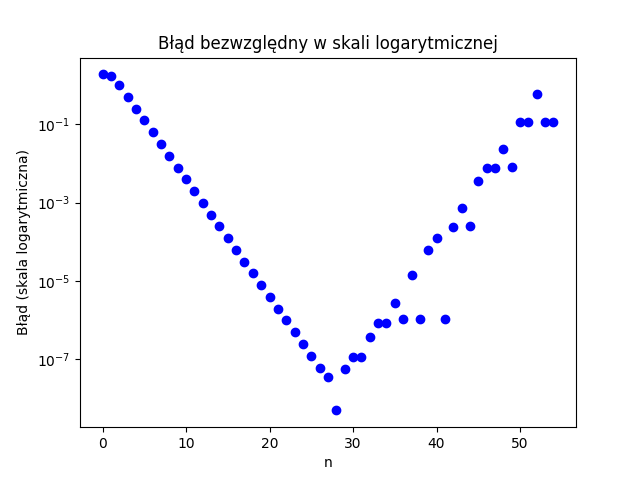
\includegraphics[width=0.7\textwidth]{../fig.png} % Adjust the width as needed
  \caption{Błąd bezwzględny od wartości n}
  \label{fig:fig1}
\end{figure}

Jak widzimy na wykresie, najmniejszy błąd jest dla $h = 2^{-28}$.
Nasz błąd potem rośnie ponieważ $2^-n$ jest na tyle małe, że dodawanie je do większego $x = 1$ sprawia, że
liczby $f(x)$ oraz $f(x + h)$ są do siebie bardzo zbliżone, a więc zarazem
nasza precyzja maleje.

\begin{figure}[H]
  \centering
  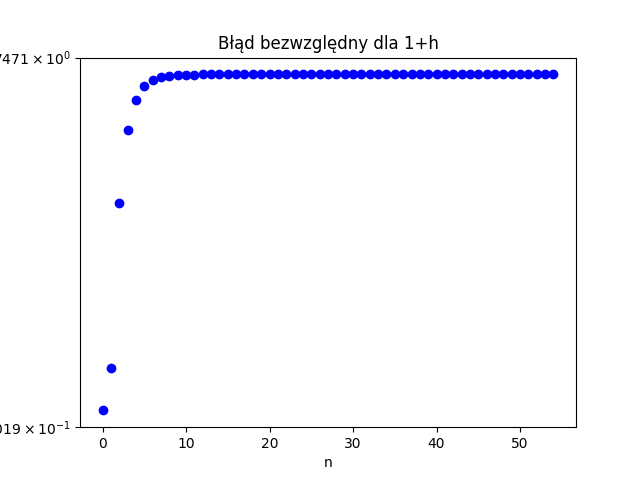
\includegraphics[width=0.7\textwidth]{../fig2.png} % Adjust the width as needed
  \caption{Błąd bezwzględny od wartości n dla $1+h$}
  \label{fig:your_label}
\end{figure}

Wiemy, że liczby są równomiernie rozłożone na przedziale $[1,2]$ co
$\delta = 2^{-52}$. Gdy do funkcji przekazujemy $1 + h$ widzimy, że
początkowo błąd rośnie aż dochodzi do $n = -52$ po czym jest stały gdyż
$h < macheps$.


\end{document}